\documentclass[runningheads]{llncs}
\usepackage{graphicx}
\usepackage{array}
\usepackage{url}

\begin{document}

\title{VaccineNLP: An Explainable Human-in-the-Loop Multi-Task NLP Framework for Vietnamese Vaccine Misinformation Surveillance}
\titlerunning{VaccineNLP: Explainable HITL Misinformation Surveillance}

\author{Manh Hung Kim\inst{1} \and Quynh Phuong Dinh Le\inst{1} \and Lam Quan Tran\inst{2} \and Hong Viet Tran\inst{3} \and Hang Nguyet Van Nguyen\inst{1}}
\authorrunning{Manh Hung Kim et al.}
\institute{Ha Noi University of Public Health, Ha Noi, Viet Nam\\ \email{2211090016@studenthuph.edu.vn} \and Digital Health Center, Ha Noi University of Public Health, Ha Noi, Viet Nam \and Institute of Artificial Intelligence, VNU University of Engineering and Technology, Vietnam National University, Hanoi, Vietnam}

\maketitle
\vspace{-0.65cm}

\begin{abstract}
Vaccine misinformation has become a public-health informatics challenge in Vietnamese digital environments, where social media posts, online comments, and informal vaccine narratives can shape vaccine confidence. This paper presents VaccineNLP, an explainable human-in-the-loop multi-task natural language processing framework for Vietnamese vaccine misinformation surveillance. We collected 1,856 Vietnamese vaccine-related texts from Facebook, YouTube, online news, Reddit, and public forums during 2020--2026, then applied an eight-step Vietnamese preprocessing pipeline and a three-axis annotation schema covering misinformation, stance, and sentiment. A 186-sample expert-validated Gold Test Set was used to compare XLM-RoBERTa, PhoBERT-v2 multi-task learning, and a Gemma-4 4B QLoRA reasoning model. PhoBERT-v2 achieved the highest average Macro F1 (0.6967), while XLM-RoBERTa obtained the best misinformation Macro F1 (0.7038) and Gemma-4 4B obtained the best sentiment Macro F1 (0.7700). Temperature Scaling reduced Expected Calibration Error by 44--56\% across the three axes. However, agreement between the LLM annotator and expert labels was very low for misinformation (Cohen's kappa = 0.0525), indicating that LLMs should support, not replace, expert medical fact-checking. Statistical tests further showed that anti-vaccine stance and negative sentiment were strongly associated with misinformation risk. The results support a cautious trustworthy-AI design for Vietnamese infodemic monitoring.

\keywords{Vaccine misinformation \and Vietnamese NLP \and Infodemic surveillance \and Human-in-the-loop \and Explainable AI \and Multi-task learning \and PhoBERT \and Confidence calibration}
\end{abstract}

\section{Introduction}
Vaccination is one of the most effective public-health interventions, yet its population-level impact depends on public trust. During and after the COVID-19 vaccine rollout, Vietnamese digital platforms became an important arena for health communication, community debate, and misinformation \cite{duong2022hesitancy,ha2022media,bui2025vaccine}. The World Health Organization describes the overabundance of accurate and inaccurate information during health crises as an infodemic, a phenomenon that requires monitoring, analysis, and timely response \cite{who2020infodemic,eysenbach2002infodemiology}.

Vaccine misinformation differs from generic fake-news detection in three important ways. First, the correctness of a claim often depends on medical evidence and public-health context rather than surface linguistic cues alone \cite{vraga2020misinformation}. Second, vaccine debates combine factual claims, stance toward vaccination, and affective framing. Third, Vietnamese online discourse contains code-switching, teen-code abbreviations, sarcasm, and evasive expressions around vaccine-related terms. These characteristics make keyword filtering insufficient for public-health surveillance.

For an international intelligent-systems audience, the paper frames the problem through three operational research questions. RQ1 asks how a Vietnamese vaccine-domain corpus can be collected, cleaned, and validated with a multi-axis annotation schema. RQ2 asks how well a Dual-Student Hybrid architecture detects misinformation while also producing interpretable explanations. RQ3 asks whether sentiment, stance, and source platform are statistically associated with misinformation risk. These questions connect model accuracy with the needs of public-health analysts who must prioritize limited review capacity during an infodemic.

The Vietnamese setting makes this problem especially relevant for EAI FISAT 2026, the EAI FPT International Conference on Intelligent Systems and Advanced Technologies, because it combines natural language processing, AI applications in healthcare, system-level implementation, comparative performance evaluation, and experimental validation. Vaccine discussions often appear as short comments, conversational fragments, or screenshots copied across platforms. A single comment may include a personal adverse event narrative, a rhetorical question, and an implicit recommendation against vaccination. For this reason, the system is designed not as a binary censorship tool, but as an intelligent surveillance and triage layer that surfaces uncertain or high-risk texts for expert review.

\subsection{Research Contributions}
This paper contributes an applied intelligent-system study at the intersection of natural language processing, trustworthy AI, health informatics, and social media analytics. The evaluation protocol addresses two aims: (i) to build and evaluate Vietnamese NLP models for vaccine-related misinformation, stance, and sentiment classification; and (ii) to assess the usefulness and limitations of LLM support for medical text annotation and explanation. To make the research contribution explicit, the paper reports four concrete outputs: C1, an expert-validated Vietnamese Gold Test Set for vaccine-related misinformation, stance, and sentiment; C2, a controlled benchmark of XLM-RoBERTa, PhoBERT-v2, and Gemma-4 4B on the same evaluation split; C3, a confidence-calibrated explainable HITL workflow for trustworthy public-health deployment; and C4, empirical evidence that LLM-based annotation remains insufficient as a replacement for expert medical fact-checking.

\section{Related Work and Research Gap}
Research on vaccine misinformation detection has progressed rapidly in English, including specialized datasets such as ANTi-Vax, where fine-tuned transformer models can reach high scores under in-domain conditions \cite{hayawi2022antivax}. Susceptibility to COVID-19 misinformation is also shaped by social-media exposure and analytic reasoning \cite{roozenbeek2020susceptibility}. However, direct transfer to Vietnamese vaccine discourse is limited by language shift, platform shift, and annotation-policy differences. Existing Vietnamese fake-news resources are useful but are generally small or not specific to vaccine and public-health communication.

The full project report identifies three concrete gaps in the Vietnamese literature. First, available Vietnamese fake-news datasets are not designed around vaccine claims, so they do not capture the difference between general political misinformation and medical misinformation. Second, prior Vietnamese NLP benchmarks rarely evaluate misinformation, stance, and sentiment under the same protocol, although these axes interact in real vaccine debates. Third, there is still limited work on Vietnamese explainable AI for health communication, where practitioners need to inspect why an item was flagged before taking action.

Transformer encoders such as BERT \cite{devlin2019bert}, XLM-RoBERTa \cite{conneau2020xlmr}, and PhoBERT \cite{nguyen2020phobert}, all built on the Transformer architecture \cite{vaswani2017attention}, are well suited to text classification because they learn contextual sentence representations. PhoBERT is particularly relevant because it is pre-trained for Vietnamese and expects word-segmented input. In contrast, decoder-only LLMs are attractive for weak annotation and natural-language explanation, but their output format can be unstable and their factual judgments in medical domains require expert oversight \cite{gilardi2023chatgpt,singhal2023medpalm}.

Table 1 positions the proposed study against related work. The table is intentionally presented as a research-positioning comparison, not as a direct leaderboard, because reported scores in the literature come from different languages, platforms, annotation policies, and class distributions. Instead, it clarifies the research gap addressed by VaccineNLP: Vietnamese vaccine misinformation has not been evaluated as a combined misinformation-stance-sentiment problem with expert validation, calibration, and operational XAI in one pipeline.

\begin{table}[t]
\caption{Research-positioning comparison of VaccineNLP against related misinformation and vaccine NLP studies.}\label{tab:literature}
\centering
\scriptsize
\setlength{\tabcolsep}{1.8pt}
\renewcommand{\arraystretch}{1.08}
\begin{tabular}{@{}>{\raggedright\arraybackslash}p{0.16\textwidth}>{\raggedright\arraybackslash}p{0.17\textwidth}>{\raggedright\arraybackslash}p{0.22\textwidth}>{\raggedright\arraybackslash}p{0.17\textwidth}>{\raggedright\arraybackslash}p{0.20\textwidth}@{}}
\hline
Study & Setting & Main task / model & Reported result & Gap addressed by VaccineNLP\\
\hline
ANTi-Vax \cite{hayawi2022antivax} & English Twitter vaccine comments & Binary vaccine misinformation detection with transformer classifiers & High in-domain F1 on a large English corpus & Not Vietnamese; binary labels do not separate misinformation, stance, and sentiment.\\
VaxxHesitancy \cite{mu2023vaxxhesitancy} & English Twitter vaccine hesitancy & Domain-specific VaxxBERT for stance and hesitancy analysis & F1 about 0.69 for hesitancy classification & Focuses on hesitancy rather than medical misinformation verification.\\
Checkovid \cite{dadgar2021checkovid} & COVID-19 misinformation on Twitter & Network and content mining with ML/NLP classifiers & Strong F1 under Twitter-based COVID-19 detection settings & Relies on Twitter-centric features; not tailored to Vietnamese vaccine discourse.\\
DANN + LIME on CoAID/MiSoVac \cite{joshi2022explainable} & Cross-platform COVID-19 misinformation & Domain adaptation plus explainable AI & Improved cross-domain F1 with LIME explanations & Explanation is model-agnostic; no Vietnamese HITL Gold Test Set or calibration analysis.\\
LLM annotation studies \cite{gilardi2023chatgpt} & General text annotation tasks & LLMs as labelers or crowd-worker alternatives & Often competitive in non-medical annotation & Medical truth claims still require expert review; our misinformation kappa was only 0.0525.\\
VaccineNLP (this study) & Vietnamese multi-source vaccine discourse & XLM-R, PhoBERT-v2 multi-task learning, Gemma-4 4B QLoRA, HITL, calibration & Mean Macro F1 = 0.6967; ECE reduced 44--56\% & Provides Vietnamese tri-axis labels, expert validation, calibrated confidence, and operational XAI.\\
\hline
\end{tabular}
\vspace{2pt}
\parbox{\textwidth}{\footnotesize\emph{Note.} Reported scores are not directly comparable because datasets, languages, label definitions, and validation protocols differ.}
\end{table}

Accordingly, Table 1 should be read as a research-positioning comparison rather than as a direct benchmark. The controlled experimental comparison is reported later in Tables 6 and 7, where XLM-RoBERTa, PhoBERT-v2, and Gemma-4 4B are evaluated on the same Vietnamese Gold Test Set under the same label schema.

The distinction between encoder and decoder models is important for this study. Encoder-only models are optimized for stable representations and classification, while decoder-only LLMs produce free-form explanations that can be useful for analysts but difficult to parse into controlled labels. This motivates the Dual-Student Hybrid architecture: PhoBERT-v2 performs routine multi-task classification, and Gemma-4 4B supports explanation for difficult cases. The design aligns with a practical division of labor instead of forcing a single model to be the classifier, annotator, fact-checker, and explainer at once.

A second gap concerns trust. Public-health AI systems must expose uncertainty and reasoning traces, not merely produce labels \cite{holzinger2019causability}. Calibration methods such as Temperature Scaling address the mismatch between model confidence and empirical correctness \cite{guo2017calibration,desai2020calibration}. Explainability methods such as Integrated Gradients and natural language rationales can make model outputs more inspectable \cite{sundararajan2017integrated}, but explanation does not guarantee factual validity. VaccineNLP therefore combines classification, calibration, and human-in-the-loop review rather than treating LLM output as ground truth.

\section{Materials and Methods}
\subsection{Data Collection and Processing}
The study uses secondary public text data and a supervised machine-learning design. The unit of analysis is a Vietnamese vaccine-related post, article, video description, or comment. Data were collected from January 2020 to March 2026 from online news, Facebook, YouTube, Reddit, and public forums. Private messages were excluded. Table 2 summarizes the source-level collection and cleaning pipeline.

Eligible texts were public Vietnamese-language items discussing human vaccination, vaccine safety, vaccine policy, adverse events, or vaccine-related trust and refusal. Exclusion criteria followed the study protocol: exact or near duplicates, spam and advertising, empty or extremely short texts, non-Vietnamese content, veterinary vaccine content, and private-channel data from platforms such as Zalo, Messenger, or Telegram. This kept the analysis focused on public discourse while reducing privacy risk.

\begin{table}[t]
\caption{Data sources and cleaning pipeline.}\label{tab:sources}
\centering
\small
\setlength{\tabcolsep}{4pt}
\renewcommand{\arraystretch}{1.05}
\begin{tabular}{lrrrrr}
\hline
Source & Initial & Deduplicated & Cleaned & Annotated & \%\\
\hline
Online news & 436 & 338 & 291 & 270 & 14.5\\
Facebook & 1,212 & 922 & 812 & 750 & 40.4\\
YouTube & 1,168 & 890 & 784 & 723 & 39.0\\
Reddit/forums & 184 & 140 & 123 & 113 & 6.1\\
Total & 3,000 & 2,290 & 2,010 & 1,856 & 100.0\\
\hline
\end{tabular}
\vspace{2pt}
\parbox{\textwidth}{\footnotesize\emph{Note.} Annotated samples are texts retained after source-level filtering, deduplication, text cleaning, and vaccine-relevance screening.}
\end{table}

The collection strategy was tier-based. Institutional sources such as online newspapers provided edited public-health communication; non-institutional sources such as Facebook, YouTube, Reddit, and forums provided community discussion; and academic or benchmark sources were used only as auxiliary references. The tier metadata allowed the analysis to compare platform risk while avoiding a false equivalence between curated news articles and informal social media comments.

The corpus followed a Bronze-Silver-Gold data architecture. The Bronze layer contained raw scraped or API-derived items. The Silver layer contained cleaned text and weak labels generated by an LLM oracle. The Gold layer contained expert-reviewed labels used for independent evaluation. After deduplication and filtering, 1,856 samples were passed to annotation; 1,496 samples were used for training, 167 for validation, and 186 for the Gold Test Set.

Vietnamese text was normalized through eight steps: HTML entity decoding, Unicode NFC normalization, URL and HTML-tag removal, hashtag splitting, emoji-to-text conversion, teen-code normalization, lowercasing, and removal of irrelevant special characters while preserving Vietnamese diacritics. Domain-specific abbreviations were expanded, for example vx to vaccine, tc to vaccination, pup to adverse reaction, and tdp to adverse effect. A relevance filter removed veterinary-vaccine and off-topic content.

The preprocessing pipeline was designed for Vietnamese social-media noise rather than formal newspaper text alone. It retained diacritics because accent removal can collapse medically meaningful tokens, but it normalized Unicode variants and conversational abbreviations. Hashtags were split into word-like units, emojis were converted into textual sentiment cues, and URLs were removed while preserving the surrounding claim. For PhoBERT-v2, the cleaned text was subsequently word-segmented so that the model received the tokenization format expected by Vietnamese pre-training.

\subsection{Annotation Schema and HITL Review}
Each sample was labeled on three axes. The misinformation axis is binary: misinformation versus correct or not evidently misleading information. The stance axis has three classes: supportive, neutral, and opposing or hesitant. The sentiment axis has three classes: positive, neutral, and negative. This separation between stance and sentiment follows the broader distinction between opinion orientation and affective polarity in sentiment analysis \cite{pang2008opinion}. Borderline cases were adjudicated by expert review, and the expert label was treated as the reference label in the Gold Test Set.

The annotation workflow combined LLM-assisted labeling with human-in-the-loop validation. A large LLM proposed initial labels and short rationales according to the codebook. Two reviewers with data-science expertise checked the structured output, and cases involving medical truth claims were reviewed under supervision from a public-health specialist. Disagreements and ambiguous texts were resolved through discussion, with the final consensus label used as the Gold Test reference. Personal post-vaccination experiences were not treated as misinformation unless they made unsupported causal claims or recommended harmful action.

\begin{table}[t]
\caption{Operational annotation schema used for HITL review.}\label{tab:schema}
\centering
\scriptsize
\setlength{\tabcolsep}{2.5pt}
\renewcommand{\arraystretch}{1.08}
\begin{tabular}{@{}>{\raggedright\arraybackslash}p{0.17\textwidth}>{\raggedright\arraybackslash}p{0.22\textwidth}>{\raggedright\arraybackslash}p{0.53\textwidth}@{}}
\hline
Axis & Label & Operational definition\\
\hline
Misinformation & Misinformation & Contains false, misleading, unsupported, or context-stripped vaccine claims.\\
Misinformation & Correct / not misleading & Consistent with available evidence or does not contain an evident misleading claim.\\
Stance & Supportive & Expresses trust, acceptance, recommendation, or encouragement toward vaccination.\\
Stance & Neutral & Provides information, asks a question, or reports an event without a clear orientation.\\
Stance & Opposing / hesitant & Expresses refusal, distrust, fear, or advice against vaccination.\\
Sentiment & Positive & Shows confidence, relief, hope, or supportive emotion.\\
Sentiment & Neutral & Does not express a clear affective polarity.\\
Sentiment & Negative & Shows fear, anger, anxiety, distrust, or blame.\\
\hline
\end{tabular}
\vspace{2pt}
\parbox{\textwidth}{\footnotesize\emph{Note.} Personal post-vaccination experience was not automatically labeled as misinformation unless it made an unsupported causal claim or harmful recommendation.}
\end{table}

After annotation and safety filtering, the modeling dataset contained 1,849 usable samples. This is seven fewer than the 1,856 texts passed to annotation because word segmentation removed malformed or empty rows. The final split preserved the study design: 1,496 training samples, 167 validation samples, and 186 expert-validated Gold Test samples (Table 4).

\begin{table}[t]
\caption{Dataset split and label counts used for training and evaluation.}\label{tab:splits}
\centering
\scriptsize
\setlength{\tabcolsep}{1.8pt}
\renewcommand{\arraystretch}{1.06}
\begin{tabular}{@{}>{\raggedright\arraybackslash}p{0.14\textwidth}>{\centering\arraybackslash}p{0.075\textwidth}>{\centering\arraybackslash}p{0.065\textwidth}>{\centering\arraybackslash}p{0.085\textwidth}>{\centering\arraybackslash}p{0.065\textwidth}>{\centering\arraybackslash}p{0.105\textwidth}>{\centering\arraybackslash}p{0.065\textwidth}>{\centering\arraybackslash}p{0.065\textwidth}>{\centering\arraybackslash}p{0.105\textwidth}>{\centering\arraybackslash}p{0.065\textwidth}@{}}
\hline
Split & N & Mis. & Corr. & Sup. & Neu-S & Opp. & Pos. & Neu-E & Neg.\\
\hline
Train & 1496 & 273 & 1223 & 427 & 622 & 447 & 303 & 571 & 622\\
Validation & 167 & 31 & 136 & 48 & 66 & 53 & 27 & 65 & 75\\
Gold Test & 186 & 28 & 158 & 54 & 84 & 48 & 40 & 75 & 71\\
Total & 1849 & 332 & 1517 & 529 & 772 & 548 & 370 & 711 & 768\\
\hline
\end{tabular}
\vspace{2pt}
\parbox{\textwidth}{\footnotesize\emph{Note.} Mis. = misinformation; Corr. = correct/not misleading; Sup. = supportive stance; Neu-S = neutral stance; Opp. = opposing or hesitant stance; Neu-E = neutral sentiment; Pos./Neg. = positive/negative sentiment. Seven samples were dropped before modeling because word segmentation removed malformed or empty rows.}
\end{table}

\subsection{Implementation Workflow}
The implementation can be summarized as a six-stage algorithmic workflow. Step 1 collects vaccine-related Vietnamese texts from news, social media, video comments, and public forums. Step 2 applies the Vietnamese preprocessing pipeline, including Unicode normalization, URL and HTML removal, hashtag segmentation, slang normalization, and word segmentation. Step 3 assigns three-axis labels for misinformation, stance, and sentiment through LLM-assisted annotation followed by HITL expert validation. Step 4 trains XLM-RoBERTa and PhoBERT-v2 classifiers and fine-tunes Gemma-4 4B with QLoRA for explanation-oriented reasoning. Step 5 evaluates all models on the expert-validated Gold Test Set using Macro F1, per-class F1, calibration error, parsing reliability, and agreement with expert labels. Step 6 deploys the calibrated PhoBERT-v2 output as the first-tier screening signal and escalates low-confidence or high-risk cases to the explanation and expert-review layer. This workflow is the operational algorithm used throughout the experiments, linking data preparation, modeling, evaluation, and human review in a single reproducible pipeline.

\subsection{Dual-Student Hybrid Architecture}
VaccineNLP adopts a Dual-Student Hybrid design. The classification engine is a PhoBERT-base-v2 shared encoder with three task-specific heads for misinformation, stance, and sentiment. The baseline is XLM-RoBERTa-base trained under comparable settings. The explanation engine is a Gemma-4 4B model fine-tuned with QLoRA to generate label-aware Vietnamese rationales \cite{dettmers2023qlora}. Figure 1 summarizes the two-tier architecture and the human-in-the-loop safety logic. The classification loss is a weighted multi-task objective:

\begin{figure}[t]
\centering
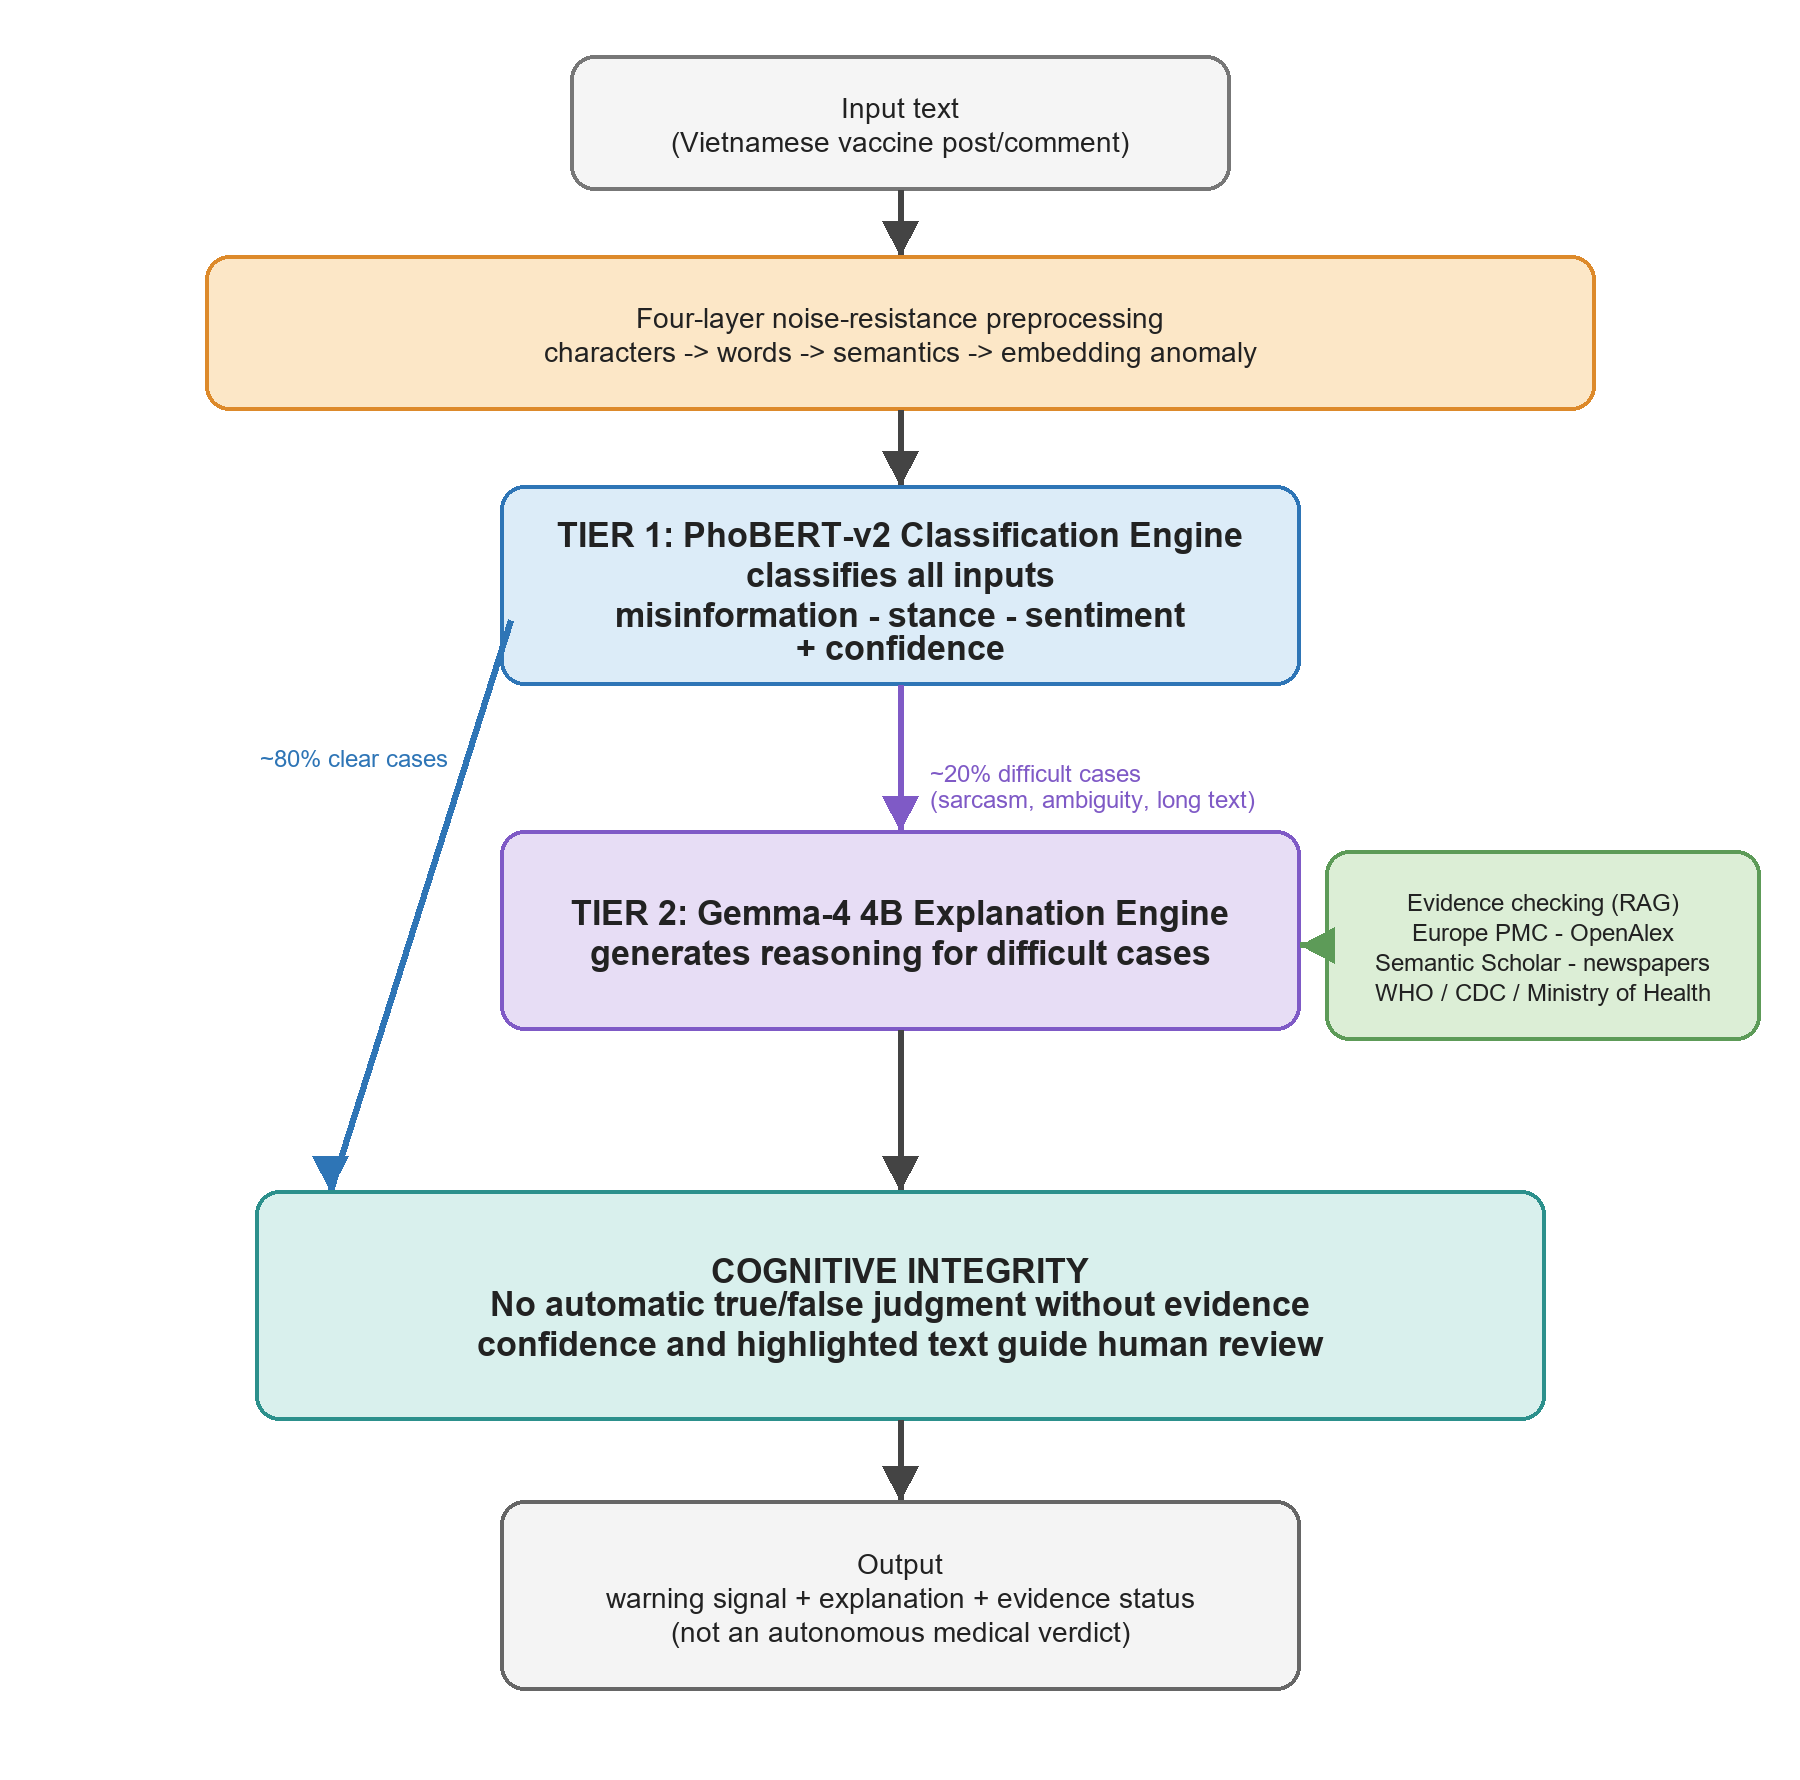
\includegraphics[width=0.78\textwidth]{figures/fig1_architecture_en.png}
\caption{VaccineNLP two-tier human-in-the-loop architecture for Vietnamese vaccine misinformation surveillance.}\label{fig:architecture}
\end{figure}

\begin{equation}
L = 1.2L_{\mathrm{misinfo}} + L_{\mathrm{stance}} + L_{\mathrm{sentiment}}.
\end{equation}

The misinformation loss was upweighted because misinformation is the minority but highest-risk class. In operational use, the classifier screens all incoming items and the reasoning engine supports explanation, triage, and expert review for high-risk or low-confidence cases.

PhoBERT-v2 used a shared Vietnamese encoder with three task-specific classification heads. The training setup followed the full report: input length was capped at 256 tokens, training batches used 16 examples, validation and test batches used 32 examples, and early stopping monitored the average Macro F1 across the three axes. XLM-RoBERTa-base was trained under a comparable split and evaluation protocol as a multilingual baseline. Weighted loss was used because the misinformation label was the minority but carried the highest public-health cost.

The encoder implementation used PhoBERT-base-v2 with a 768-dimensional pooled representation and parallel classification heads for the three annotation axes. AdamW optimization used a learning rate of 2e-5, weight decay of 0.01, three to five epochs, and a warm-up schedule of approximately 10\% of training steps. Checkpoints were selected by validation loss and monitored with Macro F1 to prevent the majority classes from dominating model selection.

Gemma-4 4B was fine-tuned with QLoRA so that a compact decoder model could generate label-aware rationales without full-parameter training. The explanation engine used longer contexts than the encoder classifier, with a maximum sequence length of 1024 tokens and an effective batch size of 16 through gradient accumulation. In the prototype, Gemma is not called for every input; it is reserved for difficult cases such as sarcasm, long conversational chains, implicit hesitation, or low calibrated confidence.

The QLoRA configuration followed the modeling experiment: 4-bit NF4 quantization, LoRA rank r = 16, LoRA alpha = 16, and text-only target modules in the attention and MLP blocks. Only about 36.7 million parameters were trainable, approximately 0.46\% of the full model. Training examples used a chat-style format in which the user message asked for vaccine misinformation analysis and the assistant response contained reasoning followed by structured labels. Loss was applied only to the response portion so the model learned to produce task-specific rationales rather than merely copy instructions.

\subsection{Evaluation Protocol and Ethics}
Classification performance was measured by Macro F1, which is appropriate for imbalanced labels \cite{he2009imbalanced}. Confidence calibration was evaluated with Expected Calibration Error before and after Temperature Scaling \cite{guo2017calibration}. Agreement between the LLM annotator and expert labels was measured by Cohen's kappa \cite{landis1977kappa}. Associations among sentiment, stance, misinformation, and source platform were tested using chi-square or G-tests with alpha = 0.05.

Temperature Scaling was fitted on the validation set and evaluated on the Gold Test Set. This method learns a single positive temperature that rescales logits before softmax, reducing overconfidence without changing the predicted class. For a public-health dashboard, this distinction matters: a calibrated confidence score supports review prioritization, whereas an overconfident but wrong prediction can mislead analysts.

The statistical tests were aligned with the pre-specified hypotheses. H1 examined the association between sentiment and stance, H2 examined the association between platform and misinformation, and H3 examined whether opposing or hesitant stance concentrated misinformation more than supportive or neutral stance. The G-test was used for platform analysis because source groups were imbalanced, while chi-square tests were used for the categorical association tables.

Error analysis was defined on randomly sampled false-positive and false-negative cases from the best-performing classifier. The error-analysis protocol grouped errors into four categories: sarcasm or irony, borderline medical content, out-of-vocabulary or emerging slang, and very short texts with insufficient context. These categories informed the future-work recommendations on sarcasm handling, active learning, and evidence-aware explanation.

The study used only publicly available text, did not collect private messages, and did not intervene on human participants. Usernames, profile URLs, phone numbers, and other potentially identifying details were removed or anonymized before analysis.

\section{Results}
The experimental results are organized so that each table answers a specific evaluation question. Table 5 describes the Gold Test Set used for evaluation. Table 6 is the primary model-comparison table: it reports task-level Macro F1 for XLM-RoBERTa, PhoBERT-v2, and Gemma-4 4B on the same expert-validated split. Table 7 provides the per-class F1 details behind those macro scores. Table 8 reports confidence calibration after Temperature Scaling, while Table 9 reports the reliability of LLM-assisted annotation against expert review. Tables 10--13 provide statistical evidence for public-health risk associations among sentiment, stance, platform, and misinformation.

The Gold Test Set contains 186 expert-reviewed Vietnamese samples. Misinformation is the minority class, with 28 samples (15.1\%), while 158 samples were labeled as correct or not clearly misleading. For stance, 54 samples were supportive, 48 opposing or hesitant, and 84 neutral. For sentiment, 71 samples were negative, 75 neutral, and 40 positive (Table 5).

\begin{table}[t]
\caption{Gold Test Set label distribution (n = 186).}\label{tab:labels}
\centering
\scriptsize
\setlength{\tabcolsep}{2.5pt}
\renewcommand{\arraystretch}{1.06}
\begin{tabular}{@{}>{\raggedright\arraybackslash}p{0.28\textwidth}>{\raggedright\arraybackslash}p{0.46\textwidth}>{\centering\arraybackslash}p{0.08\textwidth}>{\centering\arraybackslash}p{0.08\textwidth}@{}}
\hline
Axis & Class & n & \%\\
\hline
Misinformation & Correct / not misleading & 158 & 84.9\\
Misinformation & Misinformation & 28 & 15.1\\
Stance & Supportive & 54 & 29.0\\
Stance & Opposing / hesitant & 48 & 25.8\\
Stance & Neutral & 84 & 45.2\\
Sentiment & Negative & 71 & 38.2\\
Sentiment & Neutral & 75 & 40.3\\
Sentiment & Positive & 40 & 21.5\\
\hline
\end{tabular}
\end{table}

The label distribution confirms why Macro F1 was selected as the primary metric. Accuracy alone would overstate system performance because the correct/not-misleading class dominates the misinformation axis. A classifier that misses most harmful misinformation could still appear acceptable under accuracy, but would be unsafe for infodemic surveillance. Macro F1 gives each class equal weight and therefore makes minority-class weakness visible.

Table 6 is therefore the main experimental-results table for model performance. It summarizes Macro F1 across the three tasks. PhoBERT-v2 achieved the highest average Macro F1 (0.6967), suggesting that a Vietnamese-specific encoder is effective for multi-task health-text classification. XLM-RoBERTa slightly outperformed PhoBERT-v2 on the misinformation axis (0.7038 versus 0.6996), while Gemma-4 4B performed best on sentiment (0.7700), consistent with the strength of generative models in affective and contextual interpretation.

\begin{table}[t]
\caption{Primary experimental results: Macro F1 on the expert-validated Gold Test Set.}\label{tab:macro}
\centering
\small
\setlength{\tabcolsep}{4pt}
\renewcommand{\arraystretch}{1.05}
\begin{tabular}{llrrrr}
\hline
Model & Role & Misinfo & Stance & Sentiment & Mean\\
\hline
XLM-R-v1 & Baseline encoder & 0.7038 & 0.6224 & 0.6866 & 0.6709\\
PhoBERT-v2 & Classification engine & 0.6996 & 0.6640 & 0.7266 & 0.6967\\
Gemma-4 4B & XAI reasoning engine & 0.6377 & 0.6264 & 0.7700 & 0.6780\\
\hline
\end{tabular}
\end{table}

The three models therefore play complementary roles. PhoBERT-v2 is the most balanced model across tasks, with a smaller performance range between misinformation, stance, and sentiment. XLM-RoBERTa remains competitive for misinformation, possibly because its multilingual pre-training captures broader vaccine discourse. Gemma-4 4B is strongest for sentiment, but its weaker structured classification performance and parsing instability make it better suited as an explanation engine than as the sole decision engine.

The specialization pattern is also visible in the between-task Macro F1 range. The spread between the best and worst task was 0.0626 for PhoBERT-v2, 0.0814 for XLM-RoBERTa, and 0.1436 for Gemma-4 4B. This narrower range supports PhoBERT-v2 as the stable screening engine, while the wider Gemma-4 4B range supports its selective use for explanation and escalation rather than universal classification.

Per-class results show that misinformation detection remains the hardest operational task (Table 7). For the minority misinformation class, F1 was 0.5079 for XLM-RoBERTa, 0.5075 for PhoBERT-v2, and 0.4444 for Gemma-4 4B. In contrast, the correct-information class reached F1 scores close to 0.89 for the encoder models. This asymmetry reflects both label imbalance and the linguistic camouflage used in anti-vaccine content.

\begin{table}[t]
\caption{Detailed experimental results: per-class F1 by task on the Gold Test Set.}\label{tab:perclass}
\centering
\small
\setlength{\tabcolsep}{4pt}
\renewcommand{\arraystretch}{1.05}
\begin{tabular}{llrrrr}
\hline
Task & Class & XLM-R-v1 & PhoBERT-v2 & Gemma-4 4B & Support\\
\hline
Misinfo & Misinformation & 0.5079 & 0.5075 & 0.4444 & 28\\
Misinfo & Correct & 0.8997 & 0.8918 & 0.8309 & 158\\
Stance & Supportive & 0.5495 & 0.5934 & 0.4528 & 54\\
Stance & Opposing & 0.6387 & 0.6612 & 0.6905 & 48\\
Stance & Neutral & 0.6790 & 0.7375 & 0.7360 & 84\\
Sentiment & Negative & 0.7682 & 0.8000 & 0.8039 & 71\\
Sentiment & Neutral & 0.7162 & 0.7917 & 0.8034 & 75\\
Sentiment & Positive & 0.5753 & 0.5882 & 0.7027 & 40\\
\hline
\end{tabular}
\vspace{2pt}
\parbox{\textwidth}{\footnotesize\emph{Note.} F1 is reported for each class before macro-averaging within a task.}
\end{table}

\begin{figure}[t]
\centering
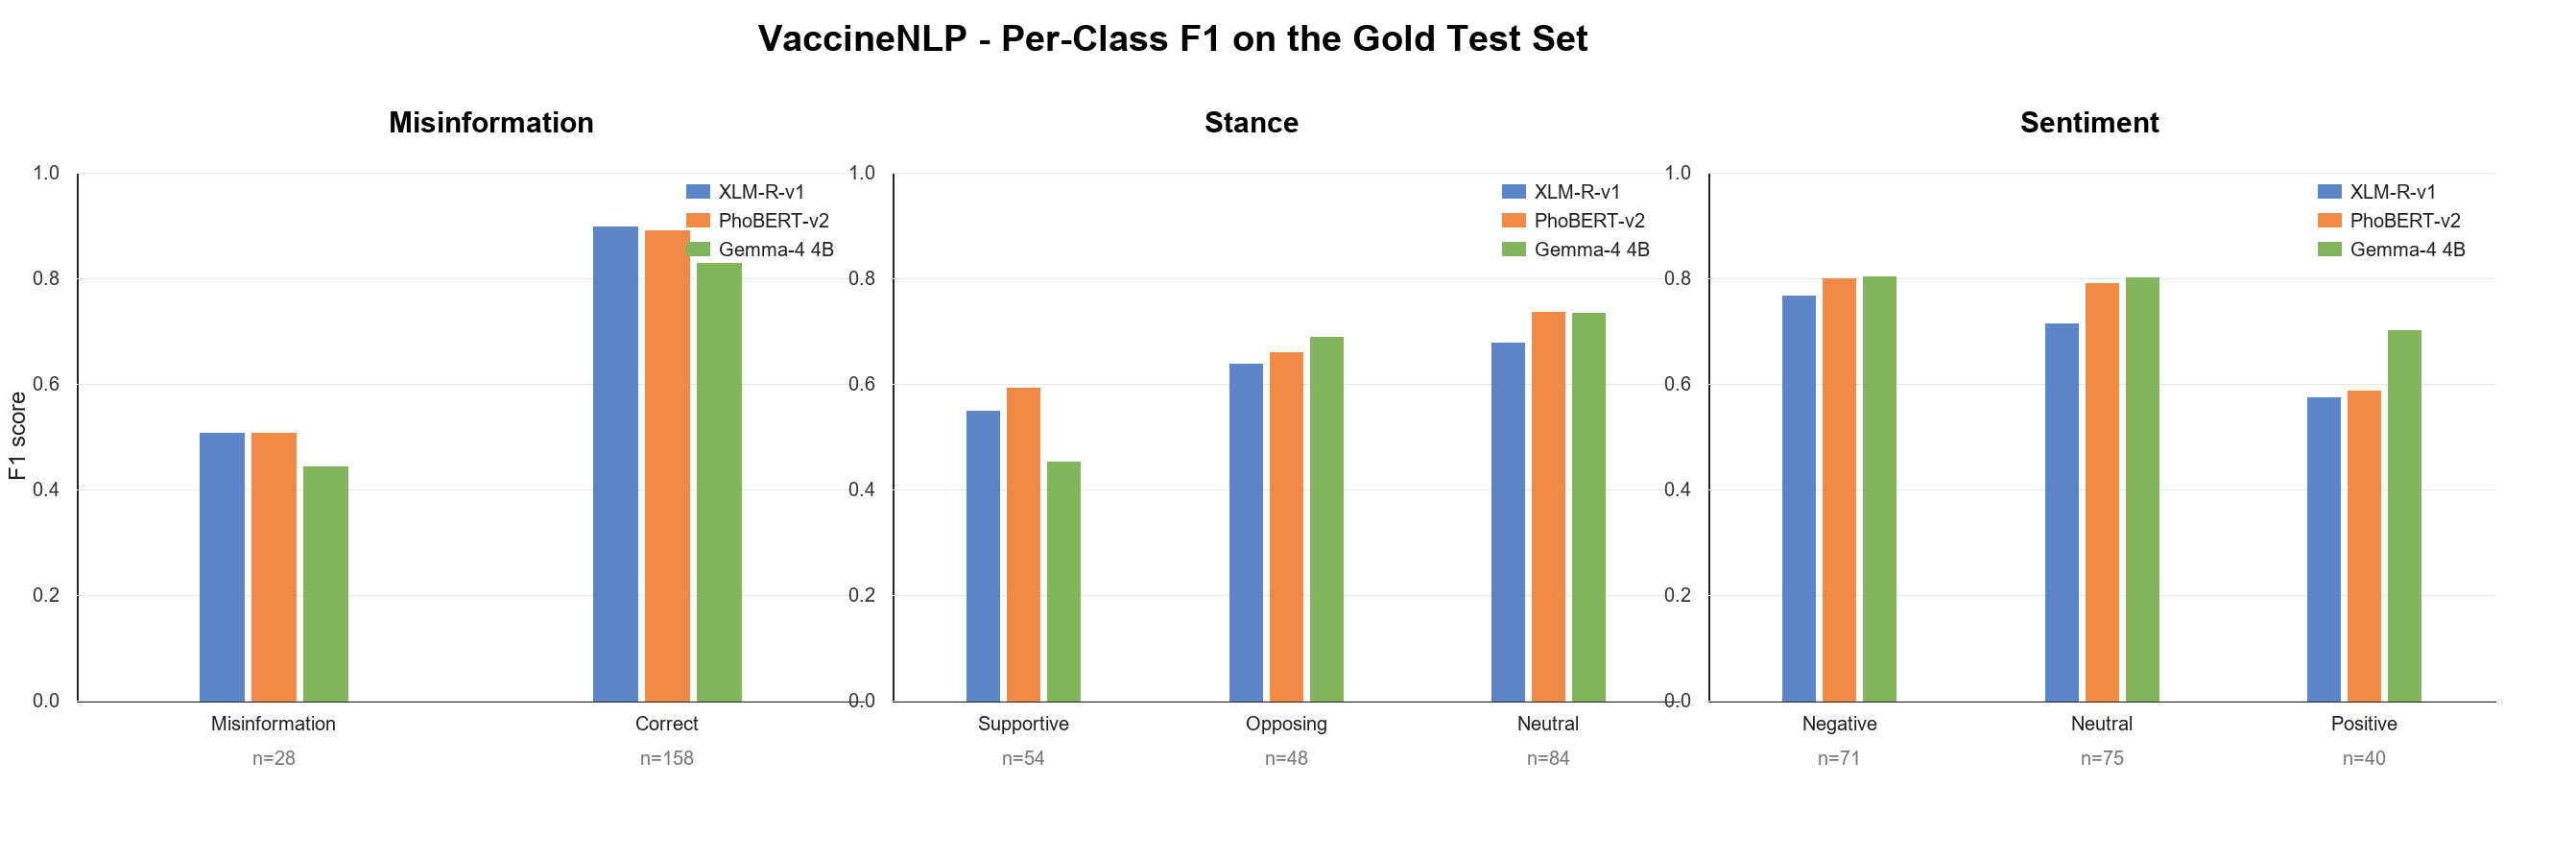
\includegraphics[width=\textwidth]{figures/fig2_per_class_f1_en.png}
\caption{Per-class F1 scores of XLM-RoBERTa, PhoBERT-v2, and Gemma-4 4B on the Gold Test Set.}\label{fig:perclass}
\end{figure}

The stance and sentiment axes show a different error profile. Neutral stance and neutral sentiment are common in news-style reporting and informational comments, while opposing stance often co-occurs with fear, distrust, or blame. Gemma-4 4B achieved strong scores on negative and neutral sentiment, which is consistent with its ability to interpret affective language, but it was less reliable on supportive stance. This pattern reinforces the value of evaluating the three axes separately rather than reporting only an aggregate score.

Temperature Scaling substantially improved confidence reliability (Table 8). For misinformation, ECE decreased from 0.123 to 0.054; for stance, from 0.198 to 0.093; and for sentiment, from 0.144 to 0.081. These reductions of 44--56\% are important for deployment because public-health analysts need calibrated risk scores, not only predicted labels.

\begin{table}[t]
\caption{Confidence calibration of PhoBERT-v2 after Temperature Scaling.}\label{tab:calibration}
\centering
\scriptsize
\setlength{\tabcolsep}{2.0pt}
\renewcommand{\arraystretch}{1.06}
\begin{tabular}{@{}>{\raggedright\arraybackslash}p{0.205\textwidth}>{\centering\arraybackslash}p{0.065\textwidth}>{\centering\arraybackslash}p{0.085\textwidth}>{\centering\arraybackslash}p{0.085\textwidth}>{\centering\arraybackslash}p{0.09\textwidth}>{\centering\arraybackslash}p{0.09\textwidth}>{\centering\arraybackslash}p{0.07\textwidth}>{\centering\arraybackslash}p{0.10\textwidth}@{}}
\hline
Axis & T & ECE pre & ECE post & Raw conf. & Cal. conf. & Acc. & ECE delta\\
\hline
Misinformation & 1.82 & 0.123 & 0.054 & 94.5\% & 87.4\% & 82.3\% & -56\%\\
Stance & 1.67 & 0.198 & 0.093 & 86.7\% & 76.3\% & 67.7\% & -53\%\\
Sentiment & 1.35 & 0.144 & 0.081 & 88.9\% & 83.0\% & 75.8\% & -44\%\\
\hline
\end{tabular}
\vspace{2pt}
\parbox{\textwidth}{\footnotesize\emph{Note.} ECE = Expected Calibration Error; T = learned temperature.}
\end{table}

\begin{figure}[t]
\centering
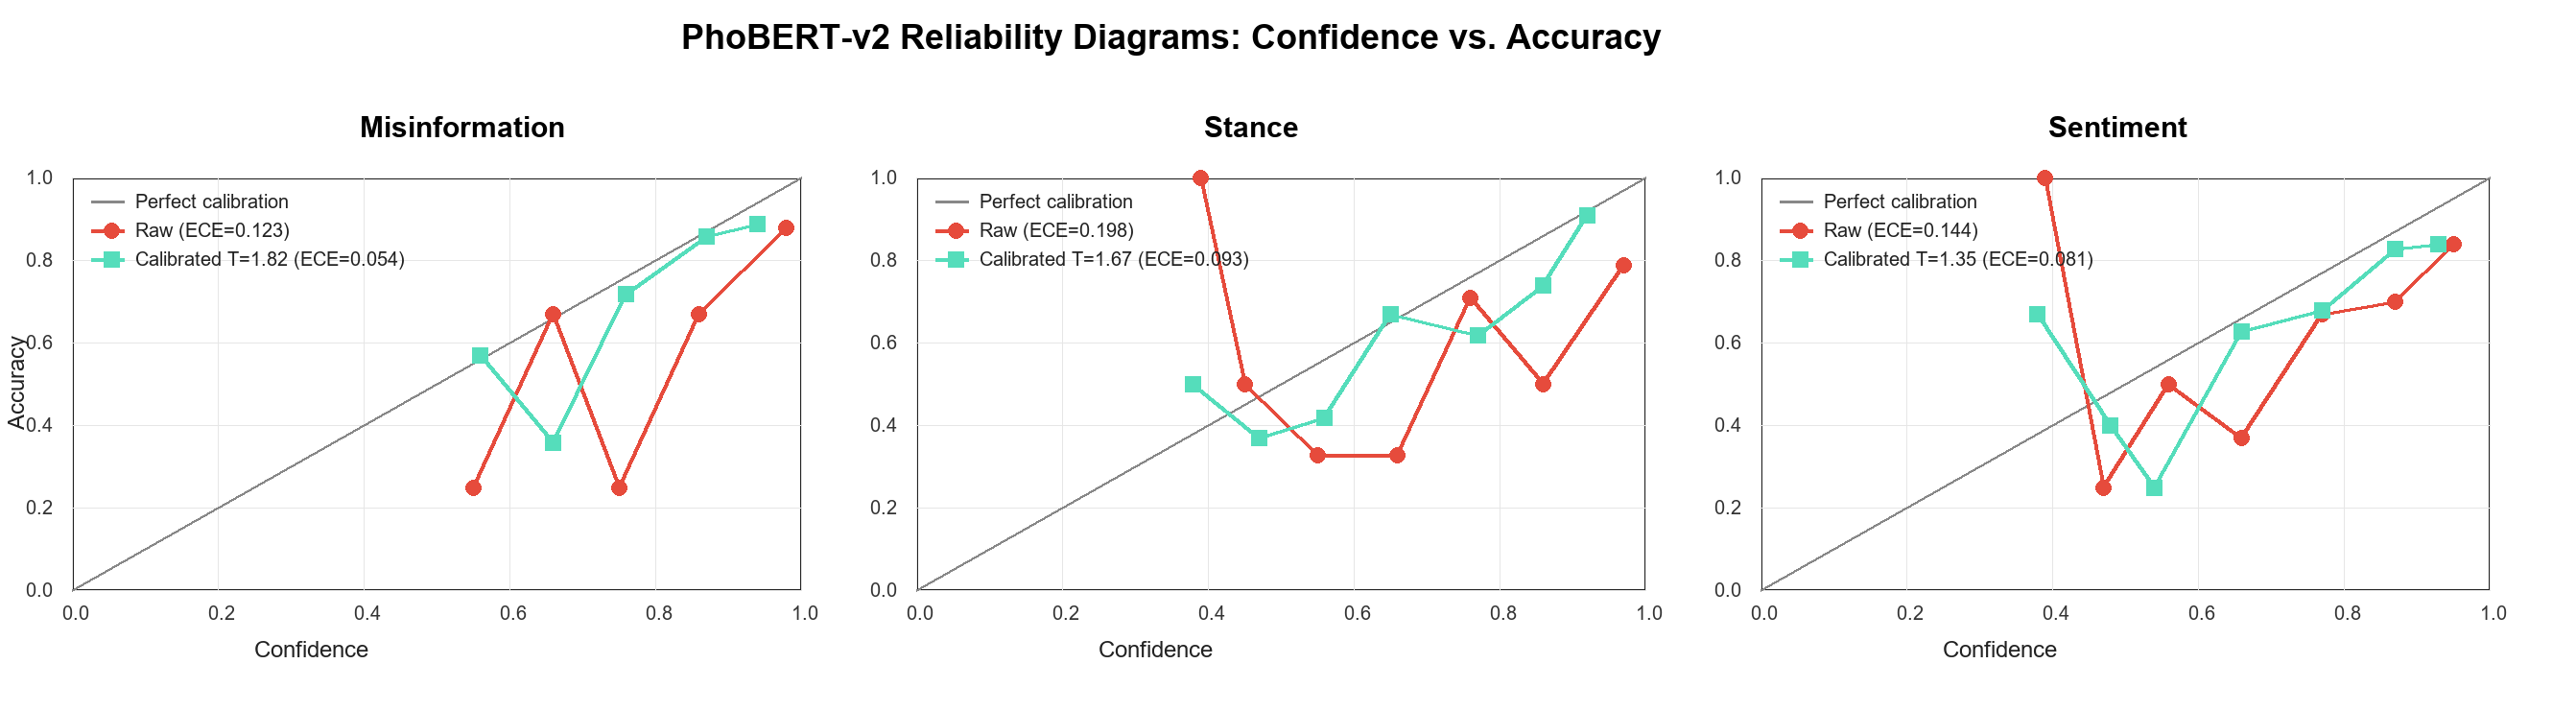
\includegraphics[width=\textwidth]{figures/fig3_calibration_en.png}
\caption{PhoBERT-v2 reliability diagrams before and after Temperature Scaling across the three tasks.}\label{fig:calibration}
\end{figure}

The calibration curves also reveal that stance is the most difficult axis to calibrate. Even after Temperature Scaling, stance ECE remains 0.093, higher than misinformation and sentiment. In practice, this means stance predictions should be displayed with explicit confidence and should trigger human review when confidence is low or when the text mixes supportive and hesitant cues.

The LLM-assisted annotation analysis exposed a major safety issue. Agreement between the LLM annotator and expert labels was very low for misinformation, fair for stance, and moderate for sentiment (Table 9). In addition, 28.0\% of Gemma-4 4B outputs on the Gold Test Set could not be parsed into the required structure. The result supports a human-in-the-loop workflow in which LLMs propose labels and rationales, but expert review remains mandatory for medical truth claims.

\begin{table}[t]
\caption{Reliability of LLM-assisted annotation against expert review.}\label{tab:llm}
\centering
\scriptsize
\setlength{\tabcolsep}{2.5pt}
\renewcommand{\arraystretch}{1.06}
\begin{tabular}{@{}>{\raggedright\arraybackslash}p{0.34\textwidth}>{\centering\arraybackslash}p{0.19\textwidth}>{\raggedright\arraybackslash}p{0.38\textwidth}@{}}
\hline
Axis / metric & Result & Interpretation\\
\hline
Misinformation kappa & 0.0525 & Slight agreement\\
Stance kappa & 0.2895 & Fair agreement\\
Sentiment kappa & 0.4712 & Moderate agreement\\
Mean kappa & 0.2711 & Low average agreement across axes\\
Invalid structured outputs & 52/186 (28.0\%) & Requires parser and human review\\
\hline
\end{tabular}
\end{table}

Parser analysis from the system evaluation shows why this matters for deployment. The improved parser handled multi-block reasoning, negation, contrastive conjunctions such as 'but' and 'however', and partial outputs when at least two of three labels were recoverable. Even with these safeguards, 52 of 186 outputs were invalid. The system therefore treats LLM explanations as auxiliary evidence and does not let a free-form rationale override expert-validated labels.

The public-health association tests were statistically significant and the cross-tabulations show where the risk concentrates. First, negative sentiment was strongly associated with anti-vaccine stance (Table 10). Among 48 opposing or hesitant samples, 45 were negative (93.8\%) and none were positive. By contrast, 38 of 54 supportive samples were positive. This pattern indicates that anti-vaccine stance is often packaged through fear, anger, distrust, or blame.

\begin{table}[t]
\caption{Cross-tabulation of sentiment and stance in the Gold Test Set.}\label{tab:sentimentstance}
\centering
\small
\setlength{\tabcolsep}{4pt}
\renewcommand{\arraystretch}{1.05}
\begin{tabular}{lrrrr}
\hline
Sentiment & Supportive & Opposing & Neutral & Total\\
\hline
Negative & 9 & 45 & 17 & 71\\
Neutral & 7 & 3 & 65 & 75\\
Positive & 38 & 0 & 2 & 40\\
Total & 54 & 48 & 84 & 186\\
\hline
\end{tabular}
\vspace{2pt}
\parbox{\textwidth}{\footnotesize\emph{Note.} The association was significant by chi-square test, chi-square = 189.48, df = 4, p = 6.85e-40.}
\end{table}

Second, platform distribution was associated with misinformation (Table 11). Facebook accounted for 19 misinformation samples among 77 Facebook samples (24.7\%), while YouTube accounted for 9 among 74 (12.2\%). The other source groups had no misinformation samples in the Gold Test Set. This does not imply that institutional media are perfect, but it does show that editorial control and public-source credibility are meaningful features for risk triage.

\begin{table}[t]
\caption{Cross-tabulation of platform and misinformation in the Gold Test Set.}\label{tab:platformmisinfo}
\centering
\scriptsize
\setlength{\tabcolsep}{2.2pt}
\renewcommand{\arraystretch}{1.06}
\begin{tabular}{@{}>{\raggedright\arraybackslash}p{0.40\textwidth}>{\centering\arraybackslash}p{0.11\textwidth}>{\centering\arraybackslash}p{0.11\textwidth}>{\centering\arraybackslash}p{0.11\textwidth}>{\centering\arraybackslash}p{0.16\textwidth}@{}}
\hline
Platform & Misinfo & Correct & Total & Misinfo rate\\
\hline
Facebook & 19 & 58 & 77 & 24.7\%\\
YouTube & 9 & 65 & 74 & 12.2\%\\
Forums / other social media & 0 & 16 & 16 & 0.0\%\\
Institutional news & 0 & 10 & 10 & 0.0\%\\
Academic / VFND & 0 & 9 & 9 & 0.0\%\\
Total & 28 & 158 & 186 & 15.1\%\\
\hline
\end{tabular}
\vspace{2pt}
\parbox{\textwidth}{\footnotesize\emph{Note.} The G-test was used as the main test because several expected counts were below five; G = 16.77, df = 4, p = 2.14e-3.}
\end{table}

Third, opposing or hesitant stance was highly concentrated with misinformation (Table 12). Twenty-four of 48 opposing samples (50.0\%) contained misinformation, compared with only 1 of 54 supportive samples (1.9\%) and 3 of 84 neutral samples (3.6\%). The opposing-versus-supportive odds ratio was approximately 53.0, a very large effect size for an applied public-health signal.

\begin{table}[t]
\caption{Cross-tabulation of stance and misinformation in the Gold Test Set.}\label{tab:stancemisinfo}
\centering
\scriptsize
\setlength{\tabcolsep}{2.2pt}
\renewcommand{\arraystretch}{1.06}
\begin{tabular}{@{}>{\raggedright\arraybackslash}p{0.36\textwidth}>{\centering\arraybackslash}p{0.12\textwidth}>{\centering\arraybackslash}p{0.12\textwidth}>{\centering\arraybackslash}p{0.12\textwidth}>{\centering\arraybackslash}p{0.17\textwidth}@{}}
\hline
Stance & Misinfo & Correct & Total & Misinfo rate\\
\hline
Supportive & 1 & 53 & 54 & 1.9\%\\
Opposing / hesitant & 24 & 24 & 48 & 50.0\%\\
Neutral & 3 & 81 & 84 & 3.6\%\\
Total & 28 & 158 & 186 & 15.1\%\\
\hline
\end{tabular}
\vspace{2pt}
\parbox{\textwidth}{\footnotesize\emph{Note.} The association was significant by chi-square test, chi-square = 61.86, df = 2, p = 3.69e-14; the opposing-versus-supportive odds ratio was approximately 53.0.}
\end{table}

Table 13 summarizes the hypothesis tests. H1 and H3 were significant at extremely small p-values, while H2 remained significant under the G-test despite the small cells in several platform groups. The results support a triage design in which negative affect, opposing stance, and high-risk platform context increase the priority of expert review.

\begin{table}[t]
\caption{Statistical tests for public-health risk associations.}\label{tab:hypotheses}
\centering
\scriptsize
\setlength{\tabcolsep}{2.0pt}
\renewcommand{\arraystretch}{1.06}
\begin{tabular}{@{}>{\centering\arraybackslash}p{0.06\textwidth}>{\raggedright\arraybackslash}p{0.25\textwidth}>{\raggedright\arraybackslash}p{0.22\textwidth}>{\centering\arraybackslash}p{0.12\textwidth}>{\centering\arraybackslash}p{0.13\textwidth}>{\centering\arraybackslash}p{0.13\textwidth}@{}}
\hline
Hyp. & Relationship & Test & Statistic & p-value & Finding\\
\hline
H1 & Sentiment x stance & Chi-square, df = 4 & 189.48 & 6.85e-40 & Reject H0\\
H2 & Platform x misinformation & G-test, df = 4 & 16.77 & 2.14e-3 & Reject H0\\
H3 & Stance x misinformation & Chi-square, df = 2 & 61.86 & 3.69e-14 & Reject H0\\
\hline
\end{tabular}
\vspace{2pt}
\parbox{\textwidth}{\footnotesize\emph{Note.} H0 denotes the null hypothesis of no association.}
\end{table}

Together, the association tests support the proposed misinformation-propagation triangle: negative affect, opposing or hesitant stance, and high-risk social platforms tend to reinforce one another. The finding does not imply that every negative comment is misinformation, nor that all Facebook or YouTube content is harmful. Instead, it gives analysts a statistically grounded triage signal for deciding which public posts should be reviewed first.

\section{Discussion}
The results indicate that Vietnamese vaccine misinformation surveillance benefits from task-specialized model roles. A Vietnamese encoder is the most stable backbone for routine classification, while a generative reasoning model is useful for interpretable explanations and sentiment-rich cases. The proposed Dual-Student Hybrid design follows a frugal and trustworthy-AI principle: use the efficient classifier for all inputs and reserve the more expensive reasoning model for cases that require explanation or human review.

This specialization is consistent with the technical nature of the tasks. Misinformation classification often requires recognizing unsupported causality, distorted evidence, or claims that are true in one context but misleading in another. Sentiment analysis, by contrast, depends more heavily on affective wording and pragmatic tone. Stance lies between these tasks because a user may express fear while still accepting vaccination, or may report an adverse event without recommending refusal. A multi-task framework is therefore more faithful to public-health communication than a single misinformation label.

Calibration should be interpreted as part of the system design, not as a post-hoc cosmetic step. In a review dashboard, the confidence score decides whether a post is routed to routine monitoring, expert review, or evidence retrieval. If the model is overconfident on ambiguous anti-vaccine content, analysts may under-review risky items. If it is overconfident on legitimate concerns, the system may discourage open discussion and reduce trust. Temperature Scaling therefore contributes to responsible deployment by aligning model confidence with observed correctness.

The implemented prototype also demonstrates how the model outputs can be exposed to public-health analysts as a review queue rather than as automatic medical truth judgments. Figure 4 illustrates the conversation-flow analysis screen, where comments are triaged with confidence signals and evidence-oriented explanations.

\begin{figure}[t]
\centering
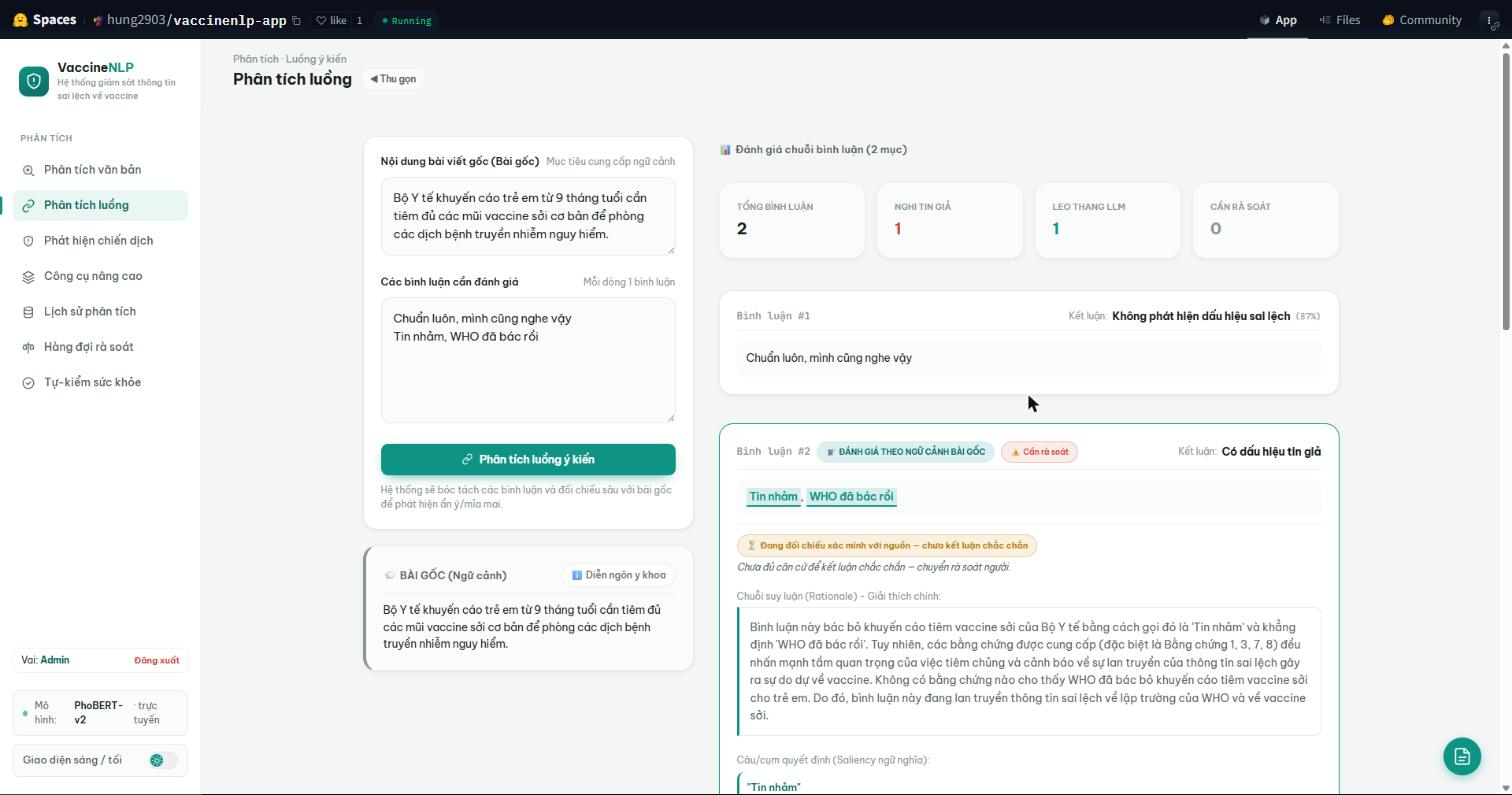
\includegraphics[width=\textwidth]{figures/fig4_prototype_stream.jpeg}
\caption{VaccineNLP prototype interface for conversation-flow screening and evidence-oriented review.}\label{fig:prototype}
\end{figure}

The prototype follows a client-server design with a web interface, an API analysis layer, model services, and persistent storage for history and review queues. The operational modules mirror the implemented system: single-text multi-task analysis, conversation-flow analysis, campaign or narrative detection, batch processing, analysis history, manual review, and system health monitoring. The classifier returns labels and softmax distributions for the three axes, while the explanation layer can add reasoning, salient text spans, and evidence status.

From a deployment perspective, the important design decision is selective escalation. Clear low-risk cases can be handled by the PhoBERT-v2 classifier, while ambiguous, sarcastic, low-confidence, or high-risk cases are escalated to the reasoning layer and then to human review. The prototype also records a consistency flag such as plausible, unusual, high-risk, or evasion-suspected. This makes the system closer to an analyst workbench than a simple demo classifier.

The proposed evidence layer combines retrieval-augmented generation with a curated public-health knowledge base. In the prototype, official sources such as WHO, CDC, and Ministry of Health guidance were treated as preferred anchors, while scientific and news sources supported broader context. This approach is important because an LLM-generated explanation can be fluent but still medically unsafe if it is not grounded in evidence.

Table 14 summarizes the deployment-oriented technical profile extracted from the project implementation. The key point is that the system was not designed as a single heavy model. It combines a lightweight Vietnamese classifier, a parameter-efficient explanation engine, calibration, structured parsing, and human review into an operational workflow for public-health monitoring.

\begin{table}[t]
\caption{Deployment-oriented technical profile of VaccineNLP.}\label{tab:deploymentprofile}
\centering
\scriptsize
\setlength{\tabcolsep}{2.0pt}
\renewcommand{\arraystretch}{1.08}
\begin{tabular}{@{}>{\raggedright\arraybackslash}p{0.22\textwidth}>{\raggedright\arraybackslash}p{0.37\textwidth}>{\raggedright\arraybackslash}p{0.32\textwidth}@{}}
\hline
Component & Evidence / configuration & Operational implication\\
\hline
PhoBERT-v2 classifier & \textasciitilde{}540 MB engine; 135M-parameter Vietnamese encoder; 256-token input; three task-specific heads & Efficient first-tier screening for all incoming vaccine-related texts\\
Gemma-4 4B QLoRA & \textasciitilde{}2.5 GB explanation engine; 4-bit NF4 QLoRA; 36.7M trainable parameters (0.46\% of the base model) & Selective rationale generation for low-confidence, sarcastic, implicit, or high-risk cases\\
Selective escalation & Prototype design escalates only difficult cases, estimated at about 20\% of inputs & Reduces computation while preserving expert oversight for ambiguous content\\
Reliability controls & Temperature Scaling reduced ECE by 44--56\%; parser v3 reached 72.0\% success (134/186) & Supports confidence-aware triage and prevents free-form LLM output from acting as ground truth\\
XAI and evidence layer & Integrated Gradients token attribution, calibrated confidence, consistency flags, and curated official-source anchors & Provides an audit trail for public-health analysts and model reviewers\\
\hline
\end{tabular}
\end{table}

The low LLM-expert agreement on misinformation is a central finding. It cautions against using LLM-generated labels as medical ground truth without validation, especially when the task requires distinguishing personal experience, outdated information, causal misinterpretation, and unsupported medical claims. In a public-health workflow, a false positive can unfairly flag legitimate concerns, while a false negative can let harmful misinformation spread through online diffusion dynamics \cite{vosoughi2018spread}.

The system also implemented token-level explanation with Integrated Gradients for PhoBERT-v2. This complements Gemma-generated rationales because it exposes which tokens contributed to the classifier output. For analysts, natural-language reasoning is easier to read; for model auditors, attribution scores are more reproducible and less prone to hallucinated justification. The combined XAI strategy is therefore not merely decorative. It gives different stakeholders different forms of inspectability.

The association results also have practical value. The combination of negative sentiment, opposing stance, and social-platform context forms a useful risk triage signal for infodemic management. Rather than treating all vaccine discussions as equal, health agencies can prioritize review queues for content where these signals converge, while still preserving expert judgment and avoiding automatic censorship-like decisions.

For Vietnamese public-health agencies, the most realistic use case is not full automation but early warning. A local CDC or digital-health team could run the classifier over public comments, rank items by misinformation risk and calibrated uncertainty, and route selected items to expert review. The system output could then inform targeted communication, FAQ updates, or community engagement. This workflow keeps accountability with trained professionals while using NLP to reduce the manual burden of monitoring thousands of posts.

\section{Limitations and Future Work}
The main limitation is the size and distribution of the Gold Test Set. With only 28 misinformation samples, minority-class F1 has a wide uncertainty range. The corpus is also dominated by Facebook and YouTube, so generalization to other platforms requires further validation. Engagement metrics such as shares, reactions, and view counts were not consistently retained after schema normalization, preventing a direct analysis of viral spread.

A second limitation is that the dataset is Vietnamese-specific and reflects the language practices of selected platforms during 2020--2026. The models may not generalize to future vaccine topics, new slang, private messaging ecosystems, or regional dialects without further annotation. The study also evaluates text-level classification; it does not reconstruct user networks, diffusion paths, or cross-platform reposting chains. These missing signals are important for measuring how misinformation actually spreads.

A third limitation concerns LLM use. Gemma-4 4B is helpful for explanations, but the parse-failure rate and low kappa on medical truth claims show that free-form LLM output is not sufficiently reliable as a labeling authority. The study therefore treats LLM labels as weak supervision and auxiliary reasoning rather than as ground truth. Future versions should enforce stricter structured decoding, run adversarial prompt tests, and compare multiple LLM families under the same expert-validated protocol.

Future work should expand expert annotation, include regional Southeast Asian multilingual data, and evaluate retrieval-augmented generation against official sources such as WHO and Vietnamese Ministry of Health guidance \cite{lewis2020rag}. Further calibration methods such as Beta Calibration or isotonic regression should be compared with Temperature Scaling, particularly for the stance axis where ECE remained 0.093 after calibration \cite{desai2020calibration}.

The next technical step is an active-learning loop. The system can select uncertain, high-impact, or disagreement-heavy samples for expert review, then periodically update the classifier and calibration layer. This would make the Gold Set grow in the areas where the model is weakest rather than sampling new data uniformly. Another direction is evidence-aware generation: rationales should be grounded in retrieved documents from WHO, CDC, the Vietnamese Ministry of Health, and peer-reviewed biomedical sources, with clear separation between model reasoning and cited evidence.

\section{Conclusion}
VaccineNLP demonstrates that multi-task Vietnamese NLP can support public-health infodemic surveillance, but only under a cautious human-in-the-loop design. PhoBERT-v2 achieved the strongest average classification performance, Temperature Scaling improved confidence reliability, and statistical tests identified meaningful links between sentiment, stance, platform, and misinformation risk. At the same time, very low LLM-expert agreement for misinformation shows that expert validation remains essential. The system is best understood as a decision-support and triage layer for public-health analysts, not an autonomous medical fact-checker.

By integrating Vietnamese-specific preprocessing, multi-axis annotation, calibrated transformer classification, LLM-assisted explanation, and statistical public-health analysis, the study provides a reproducible foundation for future Vietnamese medical NLP systems. The central lesson is practical: trustworthy vaccine misinformation surveillance requires both intelligent automation and human accountability.

\section*{Acknowledgements}
The authors thank the annotators, domain reviewers, and technical contributors who supported the VaccineNLP study, software prototype, and supporting project materials.

\bibliographystyle{splncs04}
\bibliography{references}

\section*{Correspondence and Author Contacts}
\noindent Correspondence concerning this paper should be addressed to the first author, Manh Hung Kim, Ha Noi University of Public Health, Ha Noi, Viet Nam. Email: \texttt{2211090016@studenthuph.edu.vn}.

\section*{Additional Author Contact Information}
\noindent Lam Quan Tran, Digital Health Center, Ha Noi University of Public Health, Ha Noi, Viet Nam. Email: \texttt{quantl3@fpt.edu.vn}.

\noindent Hong Viet Tran, Institute of Artificial Intelligence, VNU University of Engineering and Technology, Vietnam National University, Hanoi, Vietnam. Email: \texttt{thviet79@gmail.com}.

\end{document}
